\documentclass[a4paper,12pt]{book}


\usepackage[utf8]{inputenc}
%\usepackage[vietnam.english]{babel}

\usepackage[T1]{fontenc}




%\usepackage[Latin1]{inputenc}       %caractËres accentuÈs et autres
%\usepackage[T1]{fontenc}            %cÈsure des mots accentuÈs
%\usepackage[frenchb]{babel}         %francisation (chapitre,annexe,rÈfÈrences...)
\usepackage[top=2.5cm, bottom=3cm, left=3cm, right=3cm, headsep=14pt]{geometry}
\usepackage{graphicx}               %insertion graphiques
\graphicspath{{images/}}
\usepackage{float}
\usepackage{a4wide}
\usepackage[super]{nth}
\usepackage{mathtools}
\usepackage{hyperref}
\usepackage{fancyvrb}
\usepackage{booktabs}
\usepackage{multirow}
\usepackage{minted}
\usepackage{longtable}
\usepackage{footnote}
\usepackage{caption}
%\usepackage{psfig}


%\psfigurepath{}




%\usepackage{times}


%\input{transfig}



\renewcommand{\thefootnote}{}

%% Necessaire pour creer les index
\usepackage{makeidx}
\makeindex





%%%%%%%%%%%%%%%%%%%%%%%%%%%%%%
%%%% MODIFY THIS PART FOR THE FIRST PAGE

% change the master level 
\def\MasterLevel{Master Thesis }
%\def\MasterLevel{Master 1}

\def\InternshipTitle{Validation and Extension of an automatic framework for design space exploration of approximate variants of an application}
\def\FirstName{Nhu Khoa}
\def\LastName{Nguyen}
\def\HostOrganization{LIRMM}
\def\CityName{Montpellier}
\def\CountryName{France}
\def\UniversityName{place holder}
\def\Supervisor{Alberto Bosio}



\setlength{\textwidth}{175mm}
%
\setlength{\textheight}{245mm}

\setlength{\topmargin}{-10mm}

\setlength{\evensidemargin}{-8mm}

\setlength{\oddsidemargin}{-8mm}

% ----------------------- DEBUT DOCUMENT ---------------------------

\begin{document}



\pagestyle{plain}



\pagenumbering{Roman}


% ----------------- DEFINITION DU TITRE ET DES AUTEURS ---------------------------

\newpage
\empty
\thispagestyle{empty}

\begin{center}




%\includegraphics[angle=0,width=5cm]{images/usth-logo-final-transparent.png}



\includegraphics[angle=0,width=5cm]{images/logo-1_39.png}


\vspace*{1cm} 



{\huge University of Science and Technology of Hanoi }\\


\vspace*{1cm} 


{\large Information and Communication Technology Department}\\


\vspace*{1cm} 



{\huge \MasterLevel }\\


\vspace*{1cm} 

{\large Academic year 2017 -  2018}


\vfill


\noindent\hrulefill

\vspace*{2mm} 

{\Large \InternshipTitle }


\noindent\hrulefill





\vfill 



{\large presented by } \\

\vspace*{5mm} 


{\large \bf \FirstName~  \LastName} \\


\vspace*{5mm} 


{\large registered at \UniversityName } \\



\vspace*{5mm} 



{\large supervised by  \Supervisor } \\


\vspace*{20mm} 




{\large Host organization :   \HostOrganization }


\vspace*{5mm} 


{\large  \CityName~- \CountryName} \\

\vspace*{5mm} 





%\noindent\hrulefill


\end{center}


% ----------------------- PAGE VIDE ---------------------------




\chapter*{ATTESTATION}



\vfill


\noindent\hrulefill

~\\


I hereby,  \FirstName~  \LastName, certify that my report doesn't contain plagiarism (copy/paste) from other sources.

~\\

In case of plagiarism in my report, I know the consequences and I understand that my report won't be evaluated. In this case, my M2 internship will be noted as "fail".


~\\

 Date 

~\\
 
 Signature
 \FirstName~  \LastName
 

~\\
~\\
~\\
~\\
~\\

\noindent\hrulefill


\vfill


\vfill



%\selectlanguage{vietnam}
%
%
%Tôi ký tên dưới đây, <họ> <tên>, xác nhận rằng bài báo cáo của tôi không có đạo văn (lỗi sao chép) từ các nguồn khác.
%
%
%~\\
%
%
%Nếu bị phát hiện ra trong bài báo cáo, tôi biết hậu quả và tôi hiểu rằng bài báo cáo của tôi sẽ không được chấp nhận. 
%Trong trường hợp đó, học phần (thực tập năm thứ nhất, thực tập năm thứ hai, hay học phần đánh giá) sẽ bị ghi là “không đạt”.
%
%
%
%~\\
% 
%Ngày … tháng … năm …
% 
%
%~\\
% 
%Chữ ký
%
%
%~\\
%~\\
%~\\
%
%
%\selectlanguage{english}
%
%\noindent\hrulefill




\setcounter{page}{1}



% ----------------------- ACKNOWLEDGEMENTS ---------------------------

\chapter*{Acknowledgements}

First and foremost, I would like to express my deepest gratitude to Prof. Alberto Bosio, my research supervisor and the one who gave me this wonderful opportunity, for his patience, helpful theoretical and practical advice and enthusiastic encouragement during the period of my internship. \\
~\\
Second, I want to thank the University of Science and Technology of Hanoi (USTH) and the LIRMM Laboratory, Montpellier for granting me this opportunity to work as one of the temporary member of the lab. \\
~\\
Also, I am grateful for all the support of my colleges at LIRMM during my stay in Montpellier. \\
~\\
Last but not least, I would like to appreciate all the help and support from my family and friends during my internship. \\




% ----------------------- RESUME ---------------------------


\chapter*{Asbtract}
Convolutional Neural Network and Deep Learning is becoming popular than ever due to their great result in complex tasks such as object recognition in images/videos, natural language processing or playing sophisticated games like chess. However, they come with the cost of consuming a lot of time and energy while demand high-end hardwares.\\
In recent years, Approximate Computing(AxC) has become a major research topic in High Performance Computing in order to solve the problem of time/energy efficiency in popular computer science applications, as it focuses on trading the best precision of the calculation for less time/energy consumption, obtaining an approximated result that can still satisfy the application's need. \\
The internship emphasises on utilizing and further extending IIDEAA, an automated framework, to identify suitable portions of the Neural Network for Approximate Computing and generate variants of the source code in order to compare and choose the best version of the approximation.\\
\\
Keywords: Approximate Computing, Neural Network, Automated Framworks, High Performance Computing.

% ----------------------- PAGE VIDE ---------------------------


% ----------------------- REMERCIEMENTS ---------------------------

%\include{Thanks}

% ----------------------- TABLE DES MATIERES ---------------------------



\tableofcontents{}


\newpage


\listoffigures{}

\newpage

\listoftables


\newpage



\chapter*{List of Abreviations}


\newpage




% ----------------------- TABLE DES FIGURES ---------------------------
%\listoffigures{}

% ----------------------- TABLE DES TABLES ---------------------------
%\listoftables{}

% ----------------------- TABLE DES TABLES ---------------------------
%\listoflistings{}

% ----------------------- CHAPITRE ---------------------------
\pagenumbering{arabic}

\chapter{Introduction}

\section{Context and Motivation}
%Very brief introduction on Artificial Neural Network

Deep Learning is an approach used in the field of Artificial Intelligence and Machine Learning to help computers solve problems that are easy and intuitive for human to execute yet extremely difficult to give a formal explanation, such as object recognition. The technique centers around assisting computers in understanding the most fundamental, simplest notions of the task, building experiences and working its way through a hierarchy of concepts with increasing complexity. One of the more basic and earlier algorithms in Deep Learning is Artificial Neural Network, or Neural Network for short, which is inspired by the biological brain, thus having interconnected neurons that can receive input and produce real-value output \cite{Goodfellow-et-al-2016}. \\
~\\
%Current state of Neural Network
As of the time of writing, Artificial Neural Network, and Deep Learning in general, is becoming a trending technique in the field of Machine Learning and Artificial Intelligence, as it is being widely used and researched by many organizations. It has produced great results in complex tasks such as image recognition \cite{Krizhevsky:2012:ICD:2999134.2999257}, natural language processing \cite{recent-advances-in-deep-learning-for-speech-research-at-microsoft}, or even playing sophisticated games such as the Go game \cite{GoGame}. \\ 
~\\
%NN has disadvantages as consumes time/electricity while demands high-end hardware
While having great achievements in the past years, Deep Learning still suffers from significant drawbacks. One of its major disadvantages is being quite resource-demanding, requiring high amount of power, time and hardware capability. For example, for AlphaGo to be able to obtain its result, it cost the team 4 to 6 weeks of training the model, required 2000 CPUs and 250 GPUs which consumed 600kW of electricity. These were huge numbers, especially when compare to a 20W brain power of a Go player \cite{GoGame}. Due to this problem, researches have been conducted, both from industrial and academic side, to find an equilibrium between cost and performance. \\
~\\
%AxC might be a solution but required automated framework to be efficient
Because Artificial Neural Network has shown itself to be inherently resilient to insignificant errors, being able to use lower arithmetic precision while not hurting the overall result of the network \cite{DBLP:journals/corr/SungSH15}, Approximate Computing is a promising solution to the previously stated problem. However, due to network's high complexity, it requires a lot of time and effort to being able to explore all possible Approximate Computing variants of the neural network. Hence, an automatic framework is essential for having proficiency in finding optimal Approximated solutions. \\

\section{Internship's Objective}
In this give context, the internship at Laboratoire d'Informatique, de Robotique et de Microélectronique de Montpellier (LIRMM) focuses on the following goals: ~\\
\begin{itemize}
	\item Test and debug to improve IIDEAA, an automated framework designed to explore Approximate Computing variations of the target program.
	\item Check the framework compatibility with some C/C++ neural network library and application.
	\item Develop an automatic source-to-source mutation that will automatically generate Approximate Computing variants as the framework right now is only able to explore and test. 
\end{itemize}

\section{Host Institution - LIRMM}

Founded in 1992, LIRMM, shorts for Laboratoire d'Informatique, de Robotique et de Microélectronique de Montpellier, is a joint research laboratory between the Centre National de la Recherche Scientifique(CNRS) and the University of Montpellier. The lab has gathered many researchers from different countries, such as France, Italy, China, Brazil, and from differents institute, namely CNRS, University of Montpellier, Institut National de Recherche en Informatique et en Automatique(INRIA). \cite{LIRMM}.~\\
~\\
%LIRMM image
\begin{figure}[h]

\includegraphics[angle=0,width=11cm]{lirmm.png}
\centering
\caption{LIRMM Official Logo}
\end{figure}
~\\
Researches at LIRMM concentrate on computer science, microelectronics, and robotics that cover the following interests: Design and verify integration process, mobile and communication systems, agent-based modeling on complex systems, and studies in algorithm, bioinformatic, human-machine interactions, robotics. Research's results usually have been applied in various fields, for example, biology, telecommunication, healthcare. They are aslo used internally in the lab \cite{LIRMM}. ~\\ 
\vspace*{3cm}


\section{Report organization}

The report is organized as follow: Excluding the Introduction chapter, there are 5 chapters. The \nth{2} chapter discusses background knowledge related to Approximate Computing and one of its method, Precision Scaling. In addition, this section will also take into account the IIDEAA framework and some State of the Art that related to developing simillar framework. Chapter 3 describes the contributions made during the internship period. Testing and results are shown in the \nth{4} chapter. Last chapter will conclude the report with summary of the internship's current state, limitations faced, and possible future work. 

% ----------------------- CHAPITRE ---------------------------

\chapter{Background}

This chapter describes some background information on Approximate Computing and the automated framework IIDEAA. Section on Approximate Computing will cover its definition, motivation, challenges, and some basic strategies. As for IIDEAA, we will present two tools that the framework is made up of: Clang-Chimera, a source-to-source mutation software that apply pre-defined code mutator corresponding to some of the strategies. The other tool is an Evolution search engine named Bellerophon, which goes through Chimera's mutated source code to find the best approximated version of the program, based on how the user decide to calculate the error, reward and penalty functions.
\section{Approximate Computing}

\subsection{Definition}

Approximate computing is a computational technique that loosen up the accuracy requirement of mathematical operations performed by computers, returning a result that is possibly inaccurate (but not incorrect) compares to the exact result, yet is still within the range of "acceptable error" for an application to function properly. Such applications that enable Approximate Computing are called "error-tolerant" applications \cite{7348659}. These applications usually have gaps between the accuracy level it(or the user) require and that of the system can deliver, and thus is capitalized by Approximate Computing to produce a variety of optimizations \cite{AxCSurvey} \\
~\\
By reducing the stress of exact calculation and some minor loss of precision, this technique can promise a gain in efficiency, in terms of speed, memory, energy consumption, etc. As a prime example, the approximated version of k-mean clustering algorithm, tested by Chippa, achieved up to 50x energy reduction while losing only 5\% of accuracy and up to 5x energy reduction with insignificant error \cite{SEHD} .\\
~\\
Approximate Computing can be conducted on both hardware and software layer, providing diverse methods to apply the technique to applications. On hardware level, the target can be either: circuits, by replacing them with less accurate but more energy-efficient one, or the voltage of the hardware component, deliberately lowering it to make a compromise between accuracy and energy-consumption. With software layer, the general strategy is to overlook parts of the program that have insignificant contribution to the final result \cite{7348659}. \\

\subsection{Motivation}

Current era computing is, while advanced, without its own dilemma. Large-scale applications, namely scientific computing, social media, business and financial analysis drain far too much resources than what is available. A prediction was made that by 2020, datacenters in US will consume about 140 billion kWh of electricity, a huge increase from 91 billion kWh in 2013 \cite{NRDC}. It is clear that while computing applications are achieving incredible performance and results, the amount of resources they require is soon to be out of control as the planet's resources are limited and decreasing everyday \cite{AxCSurvey}. \\
~\\
One of the main cause of this problem is fault-free computing, which can be usually resource-intensive. The current generation computer circuit's design contains components are more vulnerable to faults and parameter variations due to low voltage supply and ever-growing integration density \cite{1322441}. Thus, for faultless computation to be used, guardbands for protection against parameter variations and error correction is apply, which increase the energy overhead tremendously \cite{7348659}. \\
~\\
Due to this fact, Approximate Computing raises as a potential solution, being the topic of interest in both industry and academic researches \cite{7348659}. Furthermore, many modern days application have inexact or noisy input, limited data precision, or are not able to find an exact output. Consequently, faultless computing becomes more redundant as rounding off results happens more often, making Approximate Computing a more optimal choice \cite{AxCSurvey}. \\

\subsection{Level of Approximate Computing}

In the article "Introduction to Approximate Computing", the author, Ben Khadra, has suggested a structure to classify all forms of development for Approximate Computing. One parameter of classification among the structure presented is the Level of Approximation, indicating which part of the system the technique is applied on. The four following categories were presented from lowest to highest respectively, in terms of cost-effective: algorithm, application, architecture, and circuit \cite{introAxC}. \\
%insert image here
~\\
Changes made at algorithm level usually are related to inputs or configuration of the algorithm while not altering the said algorithm. For application level, on the other hand, modifications to the algorithm are required. Another way to apply Approximate Computing at this level is having the ability to inspect a larger search space, for example automating the process to discover many Approximated variants of the application. Higher levels of Approximate Computing typically include adjustments to hardware, with the top-level being circuit modification. At this level, the design of the circuit is the target by changing or adding new arithmetic units, for instance adders and multipliers, which is created for approximate computing. This level is also considered as the most expensive to implement since implementations physically change the circuit into a new one \cite{introAxC}.

\subsection{Common Strategies}

\subsubsection{Precision Scaling}

As the name imply, this strategy focuses on alternating the precision/bit-width of the input or intermediate operations. Precision Scaling is usually used with Floating Point operations, and generally results in a reduction in memory requirement or computational stress. It has been revealed that by decreasing the bit-width, it allow some optimizations can be viable. One of them being reducing Floating Point operations to a much simpler, insignificant operations (such as multiply by 1) which in turns do not require a Floating Point Unit. Another is allowing the use of smaller, much faster Floating Point Unit than the typical Floating Point Unit \cite{4408271}. \\
~\\
While Precision Scaling is mainly applied to hardware layer, more specifically on architechtural level, it can still be used on software level. To perform Precision Scaling on hardware layer, one can target directly the Floating Point Unit, altering its architecture \cite{AxCSurvey}. However the same cannot be said for software layer. Without specific hardware and programming library support, it is almost impossible to do so since programmers are stuck with very basic data type, such as single-precision (32-bit) and double-precision (64-bit) floating point number. \\
~\\
Currently, with the introduction of Pascal GPU Architecture and CUDA8 API, NVIDIA has provided half-precision (16-bit) floating point number data type for computing in lower precision \cite{CUDA8}. Despite not being as in full control nor as flexible as hardware Precision Scaling, the 16-bit floating point number has made Precision Scaling strategy more viable on software level, especially how GPU has been playing an important part in modern High Performance Computing. \\

\subsubsection{Loop Perforation}

Unlike Precision Scaling which mostly aims at hardware layer, Loop Perforation explicitly targets the software layer, performing Approximate Computing by directly making changes to the application. The strategy reduces computational time(thus reducing resources consumption) by only executing only a major portion of the loop's total iterations while skipping the some of it. Loop Perforation can succeed due to the fact it takes advantage of partially redundant computations that often manifest when processing multiple inputs to acquire one output \cite{LoopPerforation}. \\

\subsection{Challenges}

Like everything that existed, Approximate Computing has its own shortcomings that limit its potential. The most noticeable drawback is the nature of the technique. Because it produces imprecise results, applications that require hard logical correctness to operate as desired are not suited to apply approximation. Examples of those are cryptography, operating system, compiler, etc. Some applications are reported to only have a limited range of input where Approximate Computing is effective \cite{AxCSurvey}. \\
~\\
Excessive use of Approximate Computing may lead to undesired behaviors that cause the program to function incorrectly. It is reported that calculating a matrix kernel with Approximate Computing applied can lead to an unsolvable solution, which blocks the program and prevents its termination \cite{AxCSurvey}. Tested by Akturk \cite{Akturk2015OnQO}, Approximate Computing, in some cases, can generate corrupted output that still passed the chosen quality metric. On top of that, in worse cases, applying the technique may cause interference with the program's synchronization process and memory ordering, and consequently produces non-deterministic results which is hard to debug.\\
~\\
Finding the right strategy for the designated program can be a daunting task. Aside from the 2 basic strategies mentioned above, there are many others to choose from, which vary in terms of scope, cost, flexibility, etc. Picking a optimal methods out of all the existing tactics proves to be difficult since they can cause different experience with different applications, and nothing can work universally. It also depends greatly on requirements and constraints imposed by the user \cite{Ansel}. \\
~\\
Another challenge that Approximate Computing must face today is the lack of automation. Up until now, Approximate Computing has played a part in the advancement of Computer Science, from lossy image compression algorithms to wireless communication. Nevertheless, manually applying this technique based on the past knowledge and experience seemed to be inefficient. Applications complexity has outgrown the 2 fore-mentioned aspects, thus rises the need for (semi)automatic frameworks that can efficiently generate approximate computing system \cite{introAxC}. \\

\section{IIDEAA Automate Framework} 

The IIDEAA framework was developed to tackle one of the challenges that is holding Approximate Computing advancement back: the absence of a general automated tool that can explore a larger possibilities of a given Approximate Computing strategy more proficient and find the best compromise between the level of inaccuracy and the efficient gained in the process. \\
~\\
The main selling point of this framework is that the user does not need to detail which part of the program to be approximated and in what way. It only asks for which functions that need to be approximated and the desired error threshold to find the best possible result. Depending on what approximate strategy is used, the framework can produce a hardware or sofware implementation of the approximated application ~\cite{iideaa}. \\
~\\
IIDEAA comprises of two smaller tools that was written in C++. The first one is Chimera, a source-to-source mutation software that can modify C/C++ source code with a given code mutator. The second tool is called Bellerophon which offers a Evolutionary Search Engine to explore the mutated code to find all the best functional approximated versions that satisfy the user's requirements. \\
%insert image of the procedure
~\\
A typical run of the framework consists of the following step: At the beginning, the user will provide to Chimera the original C/C++ source code  and the Approximate Operator that IIDEAA supports along with functions to test Approximate Computing on. At the next step, Chimera will try to mutate the source code with respect to the provided Operator, then proceed with a syntax check to ensure the mutation is successful. After that, Bellerophon will execute various version of the mutated source code by altering the mutator configuration, thus finding the best approximated version of the program. Criterion that can dictate which is the best configuration are how the error function (which calculate how much the approximated result deviate from the precise one), error threshold, and reward/penalty functions are defined. \\

\subsection{Clang-Chimera}

Chimera was written in C/C++, based on the LLVM-Clang compiler. To be able to produce source-to-source mutation, Chimera exploits a few features of the said compiler. It inspects on the Clang's Abstract Syntax Tree which is a tree-based representation of the the source code. The tree contains nodes that symbolize the langague structure of a given source code. Moreover, a set of nodes will represent a specific patterns, which illustrates a peculiar structure of the source code. \\
~\\
%example of AST
By analyzing this Abstract Syntax Tree, Chimera is able to manipulate and mutate the source code with the help of 2 existing Clang API classes: \textit{ASTMatcher} and \textit{Rewriter}. With \textit{ASTMatcher}, Chimera is able to identify which nodes to mutate based on the given mutator. After all desired nodes have been found, \textit{Rewriter} will try to apply the mutation ~\cite{iideaa}. \\

\subsection{Bellerophon}

Bellerophon takes the mutated files and mutator configurations created by Chimera as input to explore all the different possibilities based on the parameters given by the user. To exploring each possibility, Bellerophon executes the mutated application based on the corresponding configuration and estimates their performance by a set of Fitness Functions. The definition of these Fitness Functions, generally include error(accuracy loss) and reward functions, should be defined by the user so that Bellerophon can function properly. The best configurations are those that satisfy the trade-off threshold between performance and accuracy loss ~\cite{iideaa}. \\
~\\
Bellerphon takes advantages of some features of the following tools. First, it uses the ParadisEO framework, which is a metaheuristics software consisting of many evolutionary algorithm, to effectively explore approximate variants of the mutated source code and configuration. Secondly, to reduce execution time, Bellerophon uses LLVM's Just-In-Time compiler which enables the ability to translate only what is mandatory for the mutated code (e.g. part of the code that was changed) to run ~\cite{iideaa}. Since there are many variants of the mutated program to execute, if the program has to re-compile for each time a new version is being tested, it will waste a lot of time. Just-In-Time compiler solve this problem by compiling section of code that are being use repeatly (e.g. code that was not mutated) once and interpreting the mutated sections \cite{JIT}. \\

\subsection{Current Challenges}
Since IIDEAA framework was developed recently, it is still far from perfect as it still lacks a core feautre. Currently, IIDEAA framework is only able to show which is the best configurations, which is inconvenient for the user. If Bellerophon results in many configurations, manually testing all of them will take time. Ideally, IIDEAA framework should have a tool to automatically generate the variants based on achieved results. Moreover, as it has not been tested widely, bugs may still occur when running the framework, either in Chimera or Bellerophon. 

% ----------------------- CHAPITRE ---------------------------

\chapter{Contribution}

As stated in previous section, IIDEAA is a set of newly developed tools that has not been used widely. It is crucial to test out IIDEAA thoroughly to detect possible bugs and identify current limitations of the framework so that we can improve. In this testing phase, we used projects from AxBench, a benchmark designed for Approximate Computing, to see whether both tools of IIDEAA can work properly. Additionally, since one of the ambitions for IIDEAA is to apply many Approximate Computing techniques to some Artificial Neural Network libraries, compatibility with these libraries is also an issue to address. The two library that were tested are DarkNet and Fast Artificial Neural Network(FANN). \\
~\\
The last objective of this internship is to create a new tool to generate Approximate variants based on the results of the 2 other tools. However, due the time constraint and delay of the internship because of visa issue, we have only started to work on and scratched the surface of this matter.\\

\section{Testing Environment}

It is worth to mention about the environment was used to conduct all tests with IIDEAA. In this framework, both Chimera and Bellerophon required LLVM-3.9.1, which was an older version of this compiler tools (current version is 7.0.0). Other than that, Bellerophon needs ParadisEO to be installed, because it uses the engine for Evolution Searching, as pointed out in the last chapter. Ideally, we would like to install everything in a separate machine for conveniences in testing, debug and modify the source code. However, installing LLVM was a difficult task and we ran into many problems. Luckily, The developer of the framework has provided us with the option of using a Docker image. This image was based on the ArchLinux default image and has everything needed for IIDEAA to run seemlessly.\\
\vspace*{3cm}

\section{Evaluating and Debugging IIDEAA}

\subsection{Applying IIDEAA to AxBench's benchmark}

AxBench is a benchmark containing a set of applications used for various approximate computing research. The benchmark was written in C++ and has some typical application from various domain such as finance, image processing, signal processing, etc. to investigate different aspects of Approximate Computing \cite{7755728}. The benchmark comes in with implemetations for both CPU and GPU. For the sake of simplicity, we've chosen to use CPU-based application to validate IIDEAA. \\
~\\
Aside from providing configuration files with desired parameter to Chimera and Bellerophon, in order to use the sample projects from AxBench with IIDEAA, some additions and modifications have to be made to these projects. First is the inclusion of CMake, a tool designed to build, test and package software, and its config file for each project. An important note when configuring the project using CMake is that generating a \textit{compile\_command.json} is necessary. This is due to the fact that both Chimera and Bellerophon will use it later on for syntax check and compilation. For Bellerophon case, some modifications needs to be made to make sure that the compiler has the correct path to the mutated files. \\
~\\
As mentioned in previous section, the user has to define how to calculate the error causes by precision loss and the reward gained from this loss to Bellerophon. Since the error metrics for each AxBench project was made public by the development team, we have used them to implement the error function. As for the reward function, it depends on how the Approximate Operator works. For this testing phase, we used two Operators implemeted by IIDEAA's developer, VPA and VPA\_Native. The two Operators are designed for Precision Scaling strategy as they modify the precision/data type. The reward function regarding to these two Operators will be discussed in the \textit{Result and Discussion} section. \\
~\\
In addition, source code modification sometimes is required to ensure that Bellerophon will have a function that can be called to execute the main part of the program, thus producing the approximated result for each variantions of the mutated program. Lastly, the user must also have a \textit{txt} file containing the result produced by the original version of the program. Because the source code of the program is the mutated one, it is more convenient to read the original result from the text file. Also, since the comparision between both version, original and mutated, is made for every variants, having the original source ran repeatedly is time consuming. \\
~\\
All the projects that were setup to be able to run by IIDEAA are available at: \url{https://github.com/nnkhoa/IIDEAA-Bench} \\

\subsection{Bugs encountered}

While testing IIDEAA with project from AxBench, we have found a few unwanted behaviors resided in the framework, the major ones being a few cases of incorrect mutation from Chimera caused by inaccurate interpretation of the source code's Abstract Syntax Tree. Another bug found was due to overlooking type casting in calculation while mutating, thus causing ambiguity when calling parameterized constructor as the object may not have constructor implemented for arguments in such data types. \\
~\\
To demonstrate bugs regarding the mutation process, consider the following example: 
\begin{minted}[fontsize=\normalsize]{cpp}
	#define DIV 1.5
	#define TEST(X, Y) (X + Y)
	
	int k, N;
	float r;			float x, y, z;
	
	/*
	 * initialize value for the variables
	 */
	
	r =   x/y; /*(1)*/	r = (float) k/N; /*(2)*/
	r = x/DIV; /*(3)*/	r = TEST(x, y) + z; /*(4)*/
\end{minted}
The correct behavior can be expected when mutating calculation (\textit{1}) is as follow:
\begin{minted}[fontsize=\normalsize]{cpp}
	r = (float) ::vpa::VPA(x, OP_1)/::vpa::VPA(y, OP_2);
\end{minted}
In general, the mutation process will travel down the Abstract Syntax Tree, searching for specific Tree Nodes that contain paticuliar symbols, depending on the definition of the Mutation Operator. For example, in the case of VPA\_Native Operator, Chimera will look for any Binary Operators or Binary Assign Operators such as add and subtract. Once these operators are found, Chimera will attempt to make modifications on the left hand side and/or right hand sign of the operator based on the API of the Approximate Operator. \\
~\\
From the above mutation, the \verb|VPA| constructor from the VPA\_Native approximate operator takes in 2 arguments. The first one is varible of either the following type: \textit{float}, \textit{double}, \textit{long double}. The second one contains the information about the precision to be changed when execute Bellerophon. \\
~\\
However, when mutate calculation (\textit{2}), while the mutation is correct as intended from the developers, it still causes error during compilation:
\begin{minted}[fontsize=\normalsize]{cpp}
	fatal error: call to constructor of ::vpa::VPA is ambiguous
	r = (float)((float) ::vpa::VPA(k, OP_1)/::vpa::VPA(N, OP_2));
						^
\end{minted}
To breifly explain, in (\textit{2}), the implicit cast was applied to make sure the result of the division \textit{k/N}, which is the division of 2 \textit{integer},is of the same type with \textit{r} (\textit{float}, in this case). However, Chimera does not consider the implicit cast and just mutates the calculation normally as if there was no cast. Thus, it will cause a "confusion" to the compiler as VPA\_Native does not have any constructor for integer variable. \\
~\\
In the case of (\textit{3}) and (\textit{4}), since \textit{DIV} and \textit{TEST} are macros, they does not count as either variable or function, and were not properly handled, thus causing errors as below when the mutation is complete:
\begin{minted}[fontsize=\normalsize]{cpp}
	// calculation number 3
	fatal error: expected ')'
        r =(float)( ::vpa_n::VPA(x , OP_0)/ DIV;
        									   ^
	note: to match this '('
        r =(float)( ::vpa_n::VPA(x , OP_0)/ DIV;
                        ^

	// calculation number 4
	fatal error: assigning to float from incompatible type vpa_n::VPA
        r =(float)( TEST(x, y) , OP_1) +::vpa_n::VPA( z, OP_1));
          ^~~~~~~~~~~~~~~~~~~~~~~~~~~~~~~~~~~~~~~~~~~~~~~~~~~~
\end{minted}
As can be seen, the mutation finished incorrectly as there are some missing syntaxes and parenthesis compare to the normal behavior. When we tried to extract and analyze information from the Abstract Syntax Tree of these calculations, fetching names of these macros, according to the position to the Binary Operator, returned empty, thus making the Mutator has nothing to base on and does not perform any mutation. However, the Abstract Syntax Tree still recognized that these are macros. This may be reason why the mutation process ended up being incorrect. \\
~\\
There are other undedired behaviors which led to program crashes, not due to the actual source code of the framework, but because of incompatability between project's dependencies and testing environment. For example, in the \textit{Sobel} project from AxBench, it is required that the system should have \textit{Boost Library} installed. However, compilation using the library was not sucessful due to version mismatch of a depedency named \textit{icu}, which is a core component of ArchLinux Docker image. Updating this component will require a full update of the current system. However, after the update, we experienced that this has interfered with the functionality of ParadisEO and inherently, Bellerophon, making them unusable. \\

\subsection{Analyzing and Debugging}

For the problems regarding Chimera, analyze and understand how the Abstract Syntax Tree works is the one way to approach these issues. With the problem of implicit cast with calculations that concern different data types, to avoid further problems like this in the future, we assume that the variables used in the calculation all have different data types to the casting type. Because of this, we make sure that if there are any implicit cast that is detected during the mutation process, we will mutate each varible, applying the implicit cast before further mutation. 
\begin{figure}[H]
%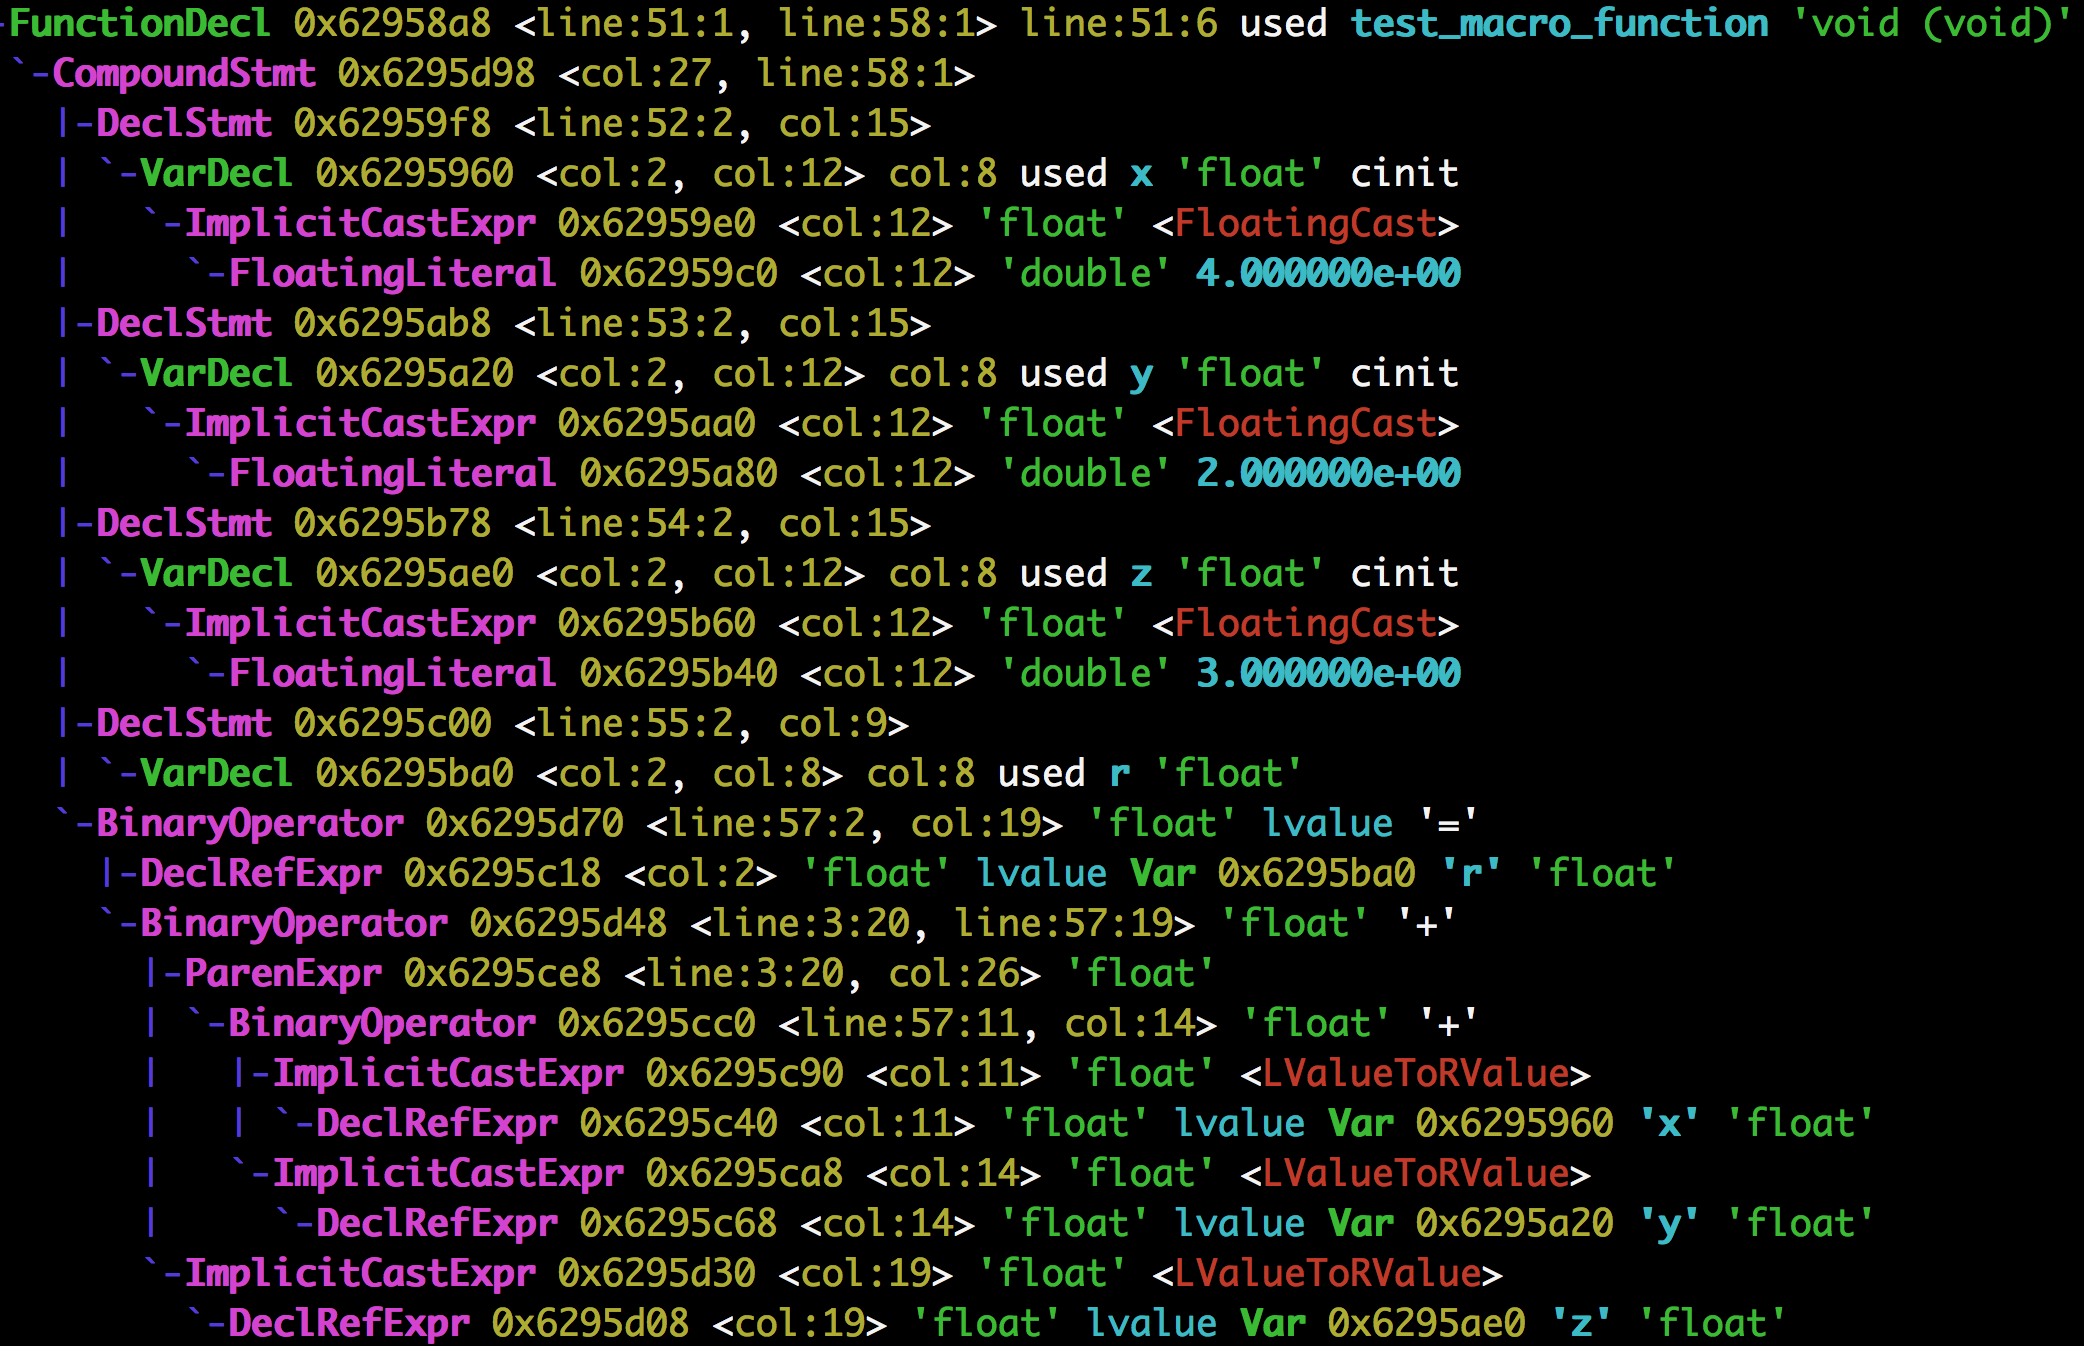
\includegraphics[width=15cm]{ast-sample.png}
\centering
\caption{Detecting Implicit Cast to decide the mutation process}
\end{figure}
This approach will ensure that even if the constructor does not have implemetation for the data type, everything will still work as expected. The result of the mutation after debugging for (\textit{2}) is as below
\begin{minted}[fontsize=\normalsize]{cpp}
	r = (float)(::vpa::VPA((float)k, OP_1)/::vpa::VPA((float)N, OP_1));
\end{minted}
Another way to deal with this problem is to modify the Approximate Operator library to have support for at least all basic data type. However, sometimes the intention is to only include an implentation for certain data type, depending on the purpose of the Approximate Operator. \\
~\\
The problem of (\textit{3}) and (\textit{4}) was a bit tricky to debug on account of the fact that some information returned by the AST is missing. In the case of (\textit{3}), as the macro is only a Literal Value, we follow the same principle as we did on the previous problem, performing check for appearances of \textit{Macro} and \textit{Literal} statement classes, then perform mutation accordingly. The same, however, can not be applied to (\textit{4}) because this is a function-like Macro with arguments which made debugging dfficult, espcially when the information returned from the Abstract Syntax Tree is missing. Currently, we do not have any solution for this problem so we try to avoid using projects or parts of the project that contains this kind of Pre-processor. The best we can do is to try and replace these function-like Macros with proper functions. \\
~\\
The debugged version of Chimera can be found at: \url{https://github.com/nnkhoa/clang-chimera}\\
\section{Compatibility with Artificial Neural Network libraries}

\subsection{Darknet}
Placeholder
\subsection{Fast Artificial Neural Network(FANN)}
Placeholder

% ----------------------- CHAPITRE ---------------------------

\chapter{Results}


This part must contain the result of the method/algoritm/system developed during the internship. \\

This part must also include comparisons with the state of the art.\\

Use tables, figures, graphics to illustrate your results. \\ 

Comment your results, and explain the context used to obtain these results.







% ----------------------- CHAPITRE ---------------------------

\chapter{Conclusion}

In the past 4 months of the internship, we were able to test the IIDEAA framework extensively, thus detected some problems around it, regarding many aspects such as the core code base, run-time issue, conflicting dependencies between run-time environment and some of the projects. From the results obtained from applying the framework to some of the AxBench's benchmark, we can further validate that choosing an suitable mutation operator is crucial when trying to utilize Approximate Computing. In addition, FANN has proven to be a Artificial Neural Network library that is compatible with IIDEAA to a certain extend. Nevertheless, further experiments might needed to see whether IIDEAA can apply Approximate Computing to everything in the library. \\
~\\
In the 2 upcoming months of the internship, we are planning to develop a tool that can generate separate variants of the mutated source code based on the result of Bellerophon. This tool will be helpful when manually editting the source code becomes infeasible due to either having large amount of acceptable results or high number of operators to modify. \\
~\\
In the future, we hope to cover all of the fore-mentioned drawbacks of IIDEAA, especially moving IIDEAA to a better run-time environment with no conflicting dependencies as well as having the latest LLVM version. Developing a new Approxmiate Operator is also desired as we would like to have more versatility within IIDEAA.\\

% ----------------------- BIBLIOGRAPHIE ---------------------------

\bibliography{Biblio}
\bibliographystyle{unsrt}

% ----------------------- ANNEXES ---------------------------

%\appendix

%\appendix

\chapter{Detail about ...}

In this part, you can add more details about some technical parts which need too much detailed impossible to include in the report body of your report








\chapter{Mathematical demonstration}

If necessary, you can add appendix to show mathematical demonstrations.





\end{document}
